\section{Grundlagen}\label{sec:grundlagen}
IEEE 802.11 mitsamt all seinen Erweiterungen ist ein äußerst umfangreicher und komplexer Standard. 
Die für das Verständnis der vorliegenden Arbeit wesentlichen Punkte werden daher in vereinfachter Form in diesem Kapitel zusammengefasst. 
Für weiterführende Informationen sei auf entsprechende Literatur (bspw. \cite{rechWLAN}) bzw. den IEEE-Standard selbst verwiesen.

\subsection{SSID, ESSID \& BSSID}
IEEE 802.11 kennt verschiedene Netzwerktopologien; grundlegend bestehen diese aus einzelnen Funkzellen, den sogenannten \textit{Basic Service Sets} (\textit{BSS}). 
Eine solche BSS verfügt über einen einzigartigen \textit{Basic Service Set Identifier} (\textit{BSSID}), welche bei den üblichen Infrastruktur-Topologien der MAC-Adresse des WLAN-Interfaces, die Funkzelle aufspannenden, \textit{Access Points} (\textit{AP}) entspricht~\cite[S. 51]{rechWLAN}. 
Besteht ein Netzwerk aus mehreren BSS-Zellen, so spricht man von einem \textit{Extended Service Set} welches über eine \textit{ESSID} verfügt. 
Diese entspricht üblicherweise dem \textit{Service Set Identifier} (\textit{SSID}) und wird in der Praxis meistens so bezeichnet. 
SSIDs können eine Länge von bis zu 32 Zeichen bzw. Byte annehmen~\cite{netgearESSID}.

\subsection{Management-Frames}
Neben den Datenframes zur Übertragung von Nutzdaten existieren im IEEE 802.11-Standard noch Kontroll- und Management-Frames. 
Kontroll-Frames dienen dabei der Steuerung des Zugriffs auf das Übertragungsmedium, Management-Frames zur Verwaltung der Funkzelle.\footcite[S. 180]{rechWLAN}

Diese drei Kategorien lassen sich weiter in einzelne Frame-Typen untergliedern. 
Die nachfolgend beschriebenen Typen fallen dabei in die Kategorie der Management-Frames. 
Ihre Übertragung erfolgt unverschlüsselt und auch unauthentifiziert, was ein Auslesen (im Fall der Probe-Requests und -Responses) sowie das Spoofen von Frames (bei Deauthentification-Frames) ermöglicht.

\subsubsection{Beacon-Frames}
Beacon-Frames werden von einem AP periodisch -- meist vielfach in einer Sekunde -- versendet, um das ausgestrahlte Netzwerk bzw. dessen Konfiguration für Stationen in Reichweite bekannt zu machen. 
Neben der SSID enthalten diese unter anderem den Kanal, auf dem der AP sendet, sowie die (Sicherheits-)Konfiguration (Übertragungsraten, verwendetes Sicherungsverfahren etc.). 
Im Fall von versteckten Netzwerken (\enquote{Hidden networks}) werden keine Beacon-Frames vom AP ausgesendet.

\subsubsection{Probe-Request- und Probe-Response-Frames}\label{subs:probes}
Mit Hilfe von Probe-Requests ist es einem Client möglich von sich aus nach Netzwerken in Reichweite zu suchen, deren SSID er kennt. 
Neben den möglichen Übertragungsraten enthält ein Probe-Request-Frame die hier wesentliche SSID des gesuchten Netzwerkes. 
Ein in Reichweite befindlicher AP, der dem über die SSID identifizierten Netzwerk zugeordnet ist, antwortet daraufhin mit einem Probe-Reponse-Frame -- allerdings nur, wenn die angegeben Übertragungsraten mit dem Netzwerk kompatibel sind. 
Aus technischer Sicht ist die Verwendung nur im Falle versteckter Netzwerke erforderlich -- die von uns in der Praxis beobachtete Sendefrequenz der Beacon-Frames ist so hoch, dass es der gezielten Nachfrage seitens des Clients nicht bedarf. 
Diese Feststellung ist wichtig, da ein Endgerät hierdurch ihm bekannte Gegenstellen verrät. 
Dadurch wird das Endgerät identifizierbar sowie anfällig für den in \ref{subs:evil-twin-attack} vorgestellten \enquote{Evil-Twin}-Angriff. 
Das Praxis-Verhalten verschiedener Geräte haben wir analysiert; Abschnitt~\ref{subs:praxisprobes} beschreibt Versuch und Ergebnisse.
%TODO: Das hier in Grundlagen zu packen sehe ich eher kritisch, nimmt viel vorweg

\subsubsection{Deauthentification-Frames}\label{subs:deauthentication-frames}
Deauthentication-Frames können vom AP (aber auch von (authentifizierten) Clients) versendet werden um eine Neuauthentifizierung des Clients beim AP anzufordern oder einfach einen bereits laufenden Authentifizierungsversuch abzubrechen. 
Gemäß der Spezifikation gibt es vielfältige Gründe (sie listet insgesamt 66 an Zahl) für das Versenden eines Deauthentification-Frames. bspw.: Inaktivität, ungültiger Schlüssel, MAC-Adresse des Clients bereits in Netz vorhanden oder aus Gründen des Load-Balancings~\cite[S. 74, S. 442]{ieee802.11}.
%TODO folgender teilsatz klingt komisch: ...durch Bewegen in eine andere Zelle des Netzwerkes und damit verbundener Wechsel des AP 
Der konkrete Grund wird dem Client durch einen sogenannten \enquote{Reason-Code} als Teil des Frames signalisiert. 
Eine solche Anweisung kann vom Client nicht ignoriert werden, da der AP die Authentifizierung schlicht widerruft und den Client damit zur Neuanmeldung zwingt (\enquote{Deauthentication is not a request; it is a notification.}~\cite[S. 74]{ieee802.11}).
 
Gerade bei Deauthentification-Frames birgt die unverschlüsselte, unauthentifizierte Übertragung ein Risiko.
So kann ein in Reichweite befindlicher Angreifer eine erneute Authentifizierung des Clients forcieren und unter Einsatz moderater Sendeleistung Angriffe gegen die Netzwerkverfügbarkeit einzelner Stationen in der Funkzelle fahren ohne im Besitz des Geheimnisses zu sein. 
Die Thematik von \textit{Denial of Service}-Angriffen mit in der Spezifikation festgelegten Frame-Typen wird bspw. in \cite{bernaschi2008access} behandelt.
%TODO: Das hier in Grundlagen zu packen sehe ich eher kritisch, nimmt viel vorweg, ist aber nicht so extrem wie oben finde ich (würde es drin lassen)

\subsection{Der Handshake bei WPA2-PSK}\label{subs:handshake}
WPA2 ist eine Implementierung des Sicherheitsstandards 802.11i welcher Authentifizierungs- und Verschlüsselungsmechanismen für die geschützte Datenübertragung in Drahtlosnetzwerken definiert.
WPA2 unterstützt zwei verschiedene Authentifizierungsmodi: 
\begin{itemize}
	\item Pre-Shared Key (PSK): Die Clients und APs teilen sich ein gemeinsames Geheimnis, dass für die Authentifizierung verwendet wird.
	\item Enterprise: Die Clients authentifizieren sich über einen RADIUS-Server. Die Anfragen werden vom AP lediglich weitergeleitet.
\end{itemize}
Folgend werden wir uns auf die Authentifizierung mit WPA2-PSK fokussieren.
Dafür wird ein sogenannter \enquote{4-Way-Handshake} zwischen dem Client (\enquote{Supplicant}) und dem AP (\enquote{Authenticator}) durchgeführt.

In einem vorbereitenden Schritt wird einmalig auf beiden Seiten der \enquote{Pairwise-Master-Key} (PMK) berechnet:
\[\mathsf{PMK} = \mathsf{PBKDF2}(\mathsf{HMAC-SHA1}, \mathsf{PSK}, \mathsf{SSID}, \mathsf{4096}, \mathsf{256})\]
Die Schlüsselableitungsfunktion PBKDF2  berechnet in 4096 Runden von HMAC-SHA1 einen 256 Bit langen Schlüssel.
Als Eingabe für den HMAC dienen der PSK als Schlüssel und die SSID als initiale Nachricht.
Nach der Berechnung des PMK kann der Handshake durchgeführt werden.
Im ersten Schritt zieht der Authenticator eine gleichverteilte\footnote{Die Noncen sollen Replay-Angriffe verhindern und werden daher zufällig gleichverteilt gezogen.} Zufallszahl, die sogenannte \enquote{ANonce}, und sendet sie an den Client.
Danach zieht der Supplicant eine eigene Zufallszahl, die sogenannte \enquote{SNonce}, und berechnet den Pairwise-Transient Key (PTK):
\[\mathsf{PTK} = \mathsf{PRF}(\mathsf{PMK}, \mathsf{Supp-MAC}, \mathsf{Auth-MAC}, \mathsf{SNonce}, \mathsf{ANonce})\]
Dafür werden der PMK, die Zufallszahlen und die MAC-Adressen beider Teilnehmer in einer Pseudozufallsfunktion (PRF) evaluiert.
Abschließend bildet der Supplicant einen Message-Integrity-Code (MIC) über seinen PTK und sendet ihn zusammen mit der SNonce an den Authenticator.
Der Authenticator besitzt nun alle Parameter um den PTK inklusive MIC zu berechnen.
Stimmt der von ihm gebildete MIC mit dem vom Supplicant übertragenen MIC überein so muss der Supplicant das korrekte Passwort kennen\footnote{Da eine Hash-Funktion zur Schlüsselableitung verwendet wird können weitere Passwörter existieren, die zum selben MIC führen.}.
In den letzten beiden Schritten werden lediglich die Schlüssel installiert und der Handshake abgeschlossen.

Abbildung \ref{fig:wpa2handshake} zeigt noch einmal anschaulich die nötigen Schritte, die während des Handshakes durchgeführt werden.
\begin{figure}[ht]
	\centering
	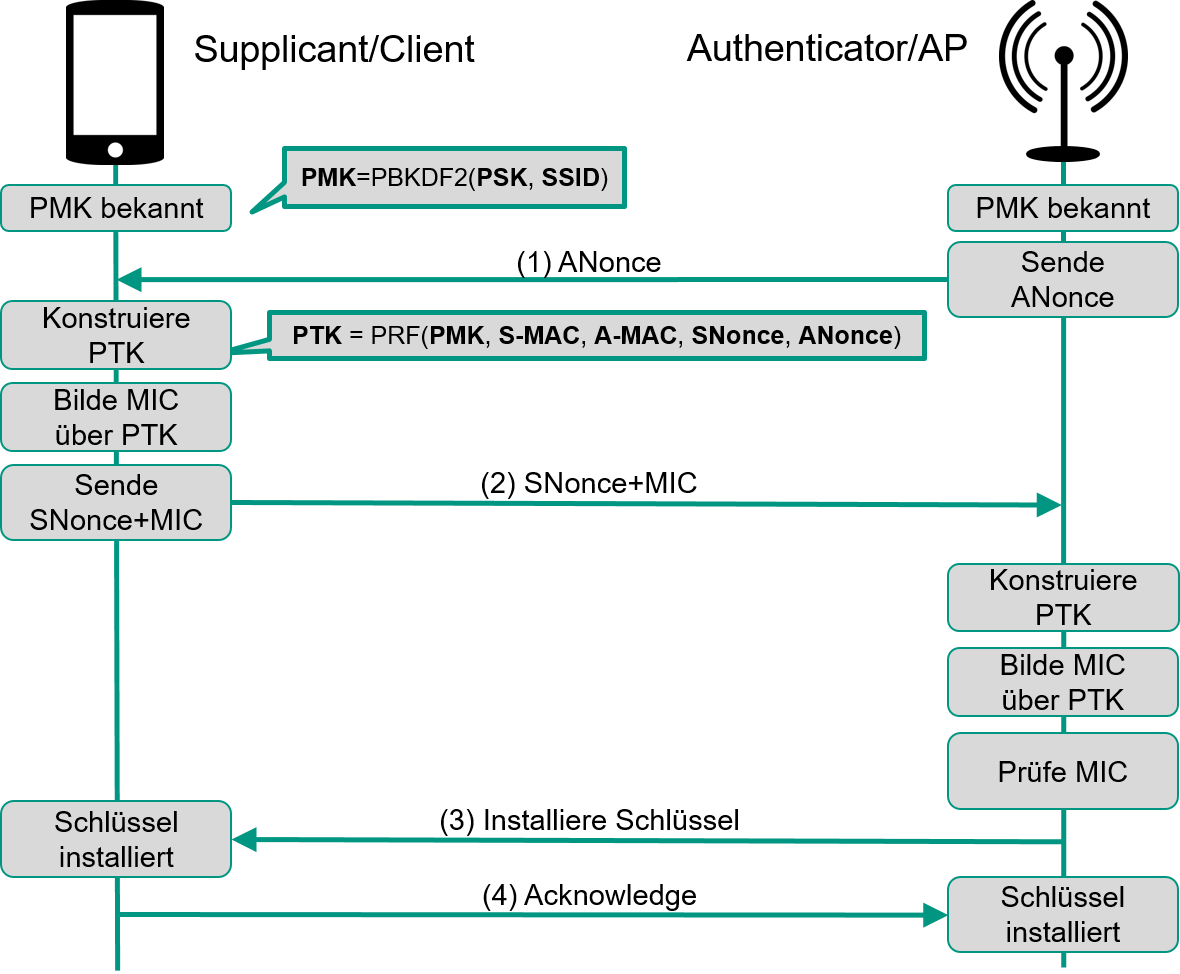
\includegraphics[width=0.80\textwidth]{graphics/wpa2handshake}
	\caption[WPA2 Handshake]{Abbildung aller vier Schritte des WPA2-Handshakes inklusive Zwischenberechnungen.}
	\label{fig:wpa2handshake}
\end{figure}

\FloatBarrier